\documentclass[border=10pt]{standalone}
\usepackage{tikz,amsmath}
\usetikzlibrary{arrows.meta}

\begin{document}
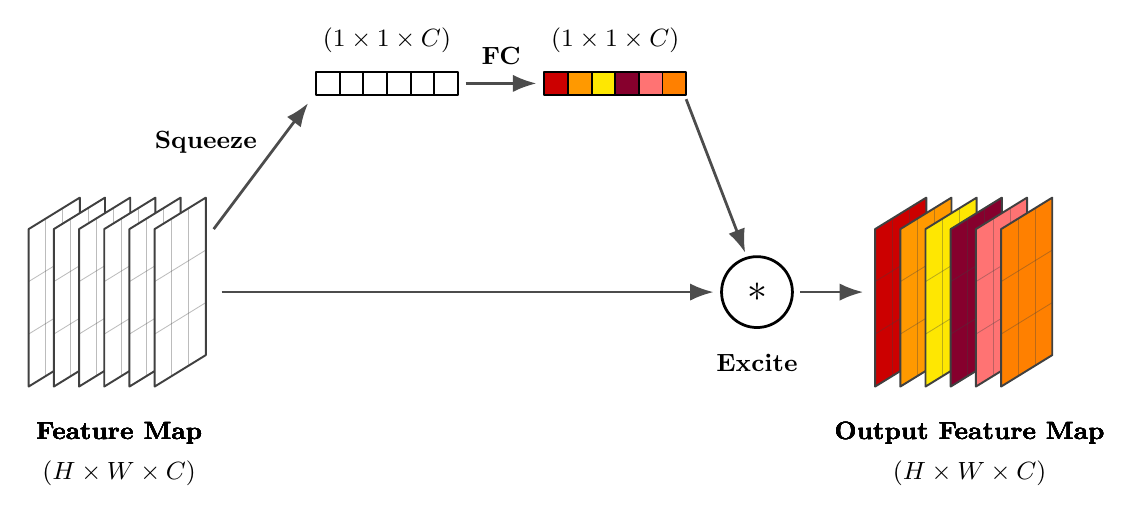
\begin{tikzpicture}[
    font=\small, line join=round,
    every node/.style={inner sep=0pt, outer sep=0pt, align=center},
    arr/.style={-{Latex[length=3mm, width=2.2mm]}, line width=1pt, black!70}
  ]

  % ========== 侧向/透视矩形特征图切片宏 ==========
  % #1: x, #2: y, #3: 填充颜色, #4: 边框颜色
  \newcommand{\tiltedslice}[4]{%
    \pgfmathsetmacro{\sw}{0.65}  % 侧向倾斜宽度
    \pgfmathsetmacro{\sh}{0.4}   % 侧向高度抬升
    \pgfmathsetmacro{\hh}{2.0}   % 特征图垂直高度
    % 切片底色填充
    \fill[#3] (#1,#2) -- ++(\sw,\sh) -- ++(0,\hh) -- ++(-\sw,-\sh) -- cycle;
    % 内部网格线 (使用 opacity 代替 !40，避免嵌套颜色语法冲突)
    \foreach \s in {1,2}{%
      \draw[#4, opacity=0.35, line width=.3pt]
        ({#1 + \s/3*\sw}, {#2 + \s/3*\sh}) -- ++(0,\hh);
      \draw[#4, opacity=0.35, line width=.3pt]
        ({#1}, {#2 + \s/3*\hh}) -- ++(\sw,\sh);
    }
    % 外侧实线边框
    \draw[#4, line width=.7pt] (#1,#2) -- ++(\sw,\sh) -- ++(0,\hh) -- ++(-\sw,-\sh) -- cycle;
  }

  % ========== 左：CNN Feature Map（6 片侧向白色矩形切片）==========
  \foreach \k in {0,...,5}
    \tiltedslice{0.75 + 0.32*\k}{1.1}{white}{black!75}
  \node[font=\small\bfseries] at (1.9,0.5) {Feature Map};
  \node at (1.9,-0) {\((H\times W\times C)\)};

  % ========== Squeeze：空的 1x1xC 条（左腿：右上斜）==========
  \draw[arr] (3.1,3.1) -- (4.3,4.7);
  \node[font=\small\bfseries] at (3.0,4.2) {Squeeze};
  \foreach \i in {0,...,5}
    \draw[black, line width=.7pt, fill=white] ({4.4+.3*\i},4.8) rectangle ++(.3,.3);
  \node at (5.3,5.5) {\((1\times1\times C)\)};

  % ========== FC：彩色权重条 ==========
  \draw[arr] (6.3,4.95) -- (7.2,4.95);
  \node[font=\small\bfseries] at (6.75,5.3) {FC};
  \foreach \col [count=\i] in {red!80!black, orange!80!yellow, yellow!90!orange,
      purple!70!black, pink!60!red, orange}
    \fill[\col, draw=black, line width=.7pt] ({7.3+.3*(\i-1)},4.8) rectangle ++(.3,.3);
  \node at (8.2,5.5) {\((1\times1\times C)\)};

  % ========== Excite：右腿右下斜，与左腿镜像 => 等腰梯形 ==========
  \draw[arr] (9.1,4.75) -- (9.85,2.8);
  \draw[arr] (3.2,2.3) -- (9.45,2.3);
  \node[circle, draw=black, line width=1pt, fill=white, minimum size=0.9cm,
        font=\Large] at (10.0,2.3) {\(\ast\)};
  \node[font=\small\bfseries] at (10.0,1.4) {Excite};

  % ========== 右：Output（6 片彩色侧向矩形切片）==========
  \draw[arr] (10.55,2.3) -- (11.35,2.3);
  \foreach \col [count=\i from 0] in {red!80!black, orange!80!yellow, yellow!90!orange,
      purple!70!black, pink!60!red, orange}
    \tiltedslice{11.5 + 0.32*\i}{1.1}{\col}{black!75}
  \node[font=\small\bfseries] at (12.7,0.5) {Output Feature Map};
  \node at (12.7,-0) {\((H\times W\times C)\)};

\end{tikzpicture}
\end{document}